\section{Protocol}
\label{sec:protocol}
To provide some context for the environment in which the proposed protocol interacts, we give some assumptions describing how we believe vulnerability disclosures and accompanying bounties are typically handled.

\subsection{Assumptions}
\subsubsection{Ethical Hacker - perspective}
\begin{enumerate}
	\item We assume it is not always as easy and/or attractive for whitehat hackers/ethical hackers to publish an exploit and retrieve an accompanying financial reward for the publication. This assumption is based on popular media such as darknet diaries, posts on news.ycombinator.com, hackernoon and possibly other sources. This assumption is based on (a combination of) the following sub-assumptions:
	\begin{enumerate}
		\item Vulnerabilities may be discovered at small/non-profit software development companies that have not allocated a large budget fraction to security.
		\item Ambiguity in the specification of the bug bounty/reward program may be interpreted in the advantage of the company during triage.
		\item The triage process may take a relatively long time, requiring the ethical hacker to have sufficient funds to sustain living costs coverage until the pay-out.
		\item A conservative/carefulness in the ethical hacker towards approaching the company with respect to the legality of discovering the vulnerability may hinder/slow down the vulnerability disclosure process.
		\item The effort required contact the company and convince them of the seriousness of the bug may consume unnecessary resources.
	\end{enumerate}
\end{enumerate}

\subsubsection{Company - perspective}
\begin{enumerate}
	\item We assume cybersecurity vulnerabilities become increasingly more relevant in our increasingly more digitized world. This assumption may be seen as being substantiated by for example the \textit{Cyber Security Assessment Netherlands 2021 (CSAN 2021)} as presented by the Dutch National Coordinator Counterterrorism and Safety of the Ministry of Justice and Security. Currently, there is only the Dutch version available at: \url{https://www.nctv.nl/onderwerpen/cybersecuritybeeld-nederland/documenten/publicaties/2021/06/28/cybersecuritybeeld-nederland-2021}. We assume that this trend can be extrapolated from a Dutch perspective to a more global perspective, given the international media coverage of for example many ransomware attacks.
	\item We assume that companies are interested, or will become more interested, in showing their customers and/or stakeholders (a quantified perspective on) \textit{how} secure their technology is. We assume it can be quite challenging to convey this perspective clearly due to the following factors:
	\begin{enumerate}
		\item Vulnerabilities can be found in various sections of the company, ranging from social engineering, misconfiguration to zero-day exploits. It is difficult to give customers a comprehensive yet concise/simple insight in how "secure" all these attack surfaces are.
		\item The impact of a vulnerability may be ambiguous or not easily quantifiable. For example, for some companies, vulnerabilities may allow malicious actors to take over critical infrastructure, whilst other vulnerabilities may lead to dataleaks or other undesired side effects.
		\item It may be difficult to accurately assess the capabilities of malicious adversaries.
	\end{enumerate}
	\item We assume some companies might be unfamiliar with vulnerability disclosure and accompanying triage processes, these delicate processes may seem intimidating for new companies that want to start paying attention to their cybersecurity, and this may lead to a lower allocation of cybersecurity budget. \textit{Note, this assumption is based entirely on imagination, no real world evidence has been found that this is indeed the case.}
\end{enumerate}


\subsection{Solution}
For a specific type of vulnerability, some, to all of these concerns can be alleviated. The scope/applicability of the protocol is visualised in \cref{fig:protocol_scope}.
\begin{figure}[H]
    \centering
    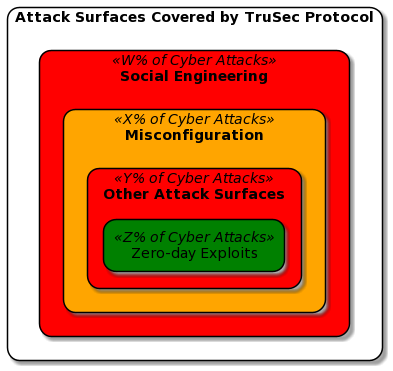
\includegraphics[width=0.50\textwidth]{images/plantuml/scope.png}
    \caption{(See notes) The proposed TruSec protocol is not suited to deal with social engineering attacks, nor is it ideal for misconfiguration exploits and/or supply-chain attacks. Instead, it is designed to increase the rate of discovery of zero day exploits. Note, we acknowledge that attacks can, in practice, also be a combination of the types.}
    \label{fig:protocol_scope}
\end{figure}

\noindent With this scope defined, one can look at how companies and ethical hackers interact according to the proposed protocol. This is visualised in \cref{fig:interaction}.

\begin{figure}[H]
    \centering
    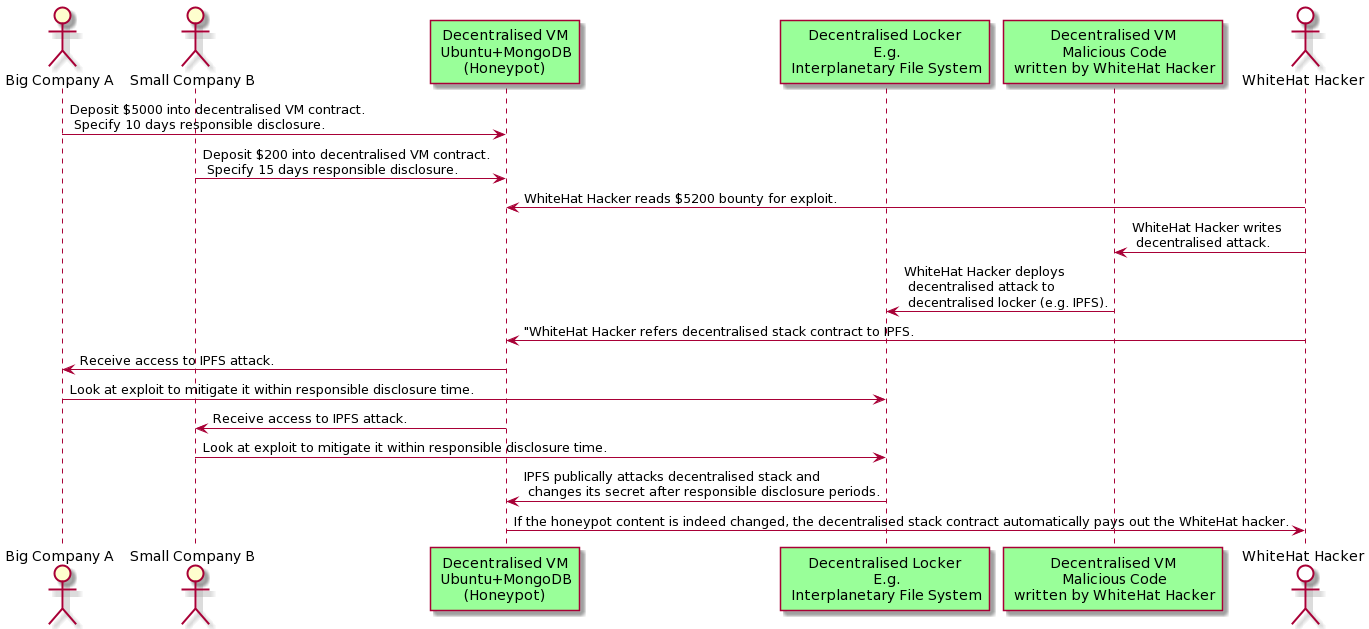
\includegraphics[width=1.0\textwidth]{images/plantuml/interaction.png}
    \caption{(See notes) Rough sketch describing the interaction of the TruSec protocol. This is an ever-lasting cycle, where at the end of the process, companies can re-deploy the patched decentralised stack, and allocate new funds. Whitehat hackers can scan for new attacks.}
    \label{fig:interaction}
\end{figure}
\noindent So the basic idea is that companies can put their open source stacks on a decentralised virtual machine (honeypot), then collectively stake money on the stacks, such that everyone can see how much money says: \textit{the use of certain software packages/combinations is safe}. This enables companies, e.g. company $A$, to show their customers for example:

\textit{With us, your data is stored using MongoDB Version 5.1, \$314.159,- says it is uncompromised, and it's running on Ubuntu Server version 21.10, which has \$4.200.000,- staked on its security. This setup has a configuration with a security on which we staked \$9001,-. If any of these software packages get compromised by whitehat hackers, we will be the first to know.}

We believe that might be clear language that enables decision makers and customers interested in company $A$, to get an intuitive understanding on \textit{how secure} some (critical) segments of the company $A$ software is.

For the whitehat/ethical hackers, the advantages are clear; they know before they start their work how large their payout will be, and they get a direct payout upon completion (after the predetermined responsible disclosure period has ended).

Note. We are aware that the TruSec protocol does not provide a clear picture on the complete security of a system/company, since a chain is only as strong as its weakest link. Hence, if other attack surfaces, such as social engineering are used, companies can still get compromised, regardless of the amount they staked. Therefore, it is important that the numerical value of the amount staked on the zero-day exploit security level is not abused to convey a false sense of security by the staking companies to their customers. Nevertheless, we think for the zero-day-exploit the amounts staked on certain systems and/or configurations, may provide an improved insight.
\subsection{\Cref{fig:protocol_scope} notes}
With respect to \cref{fig:protocol_scope}, the following notes are made:
\begin{enumerate} 
    \item The orange attack types imply the proposed protocol is not designed to tackle these issues, nor does it provide full coverage (against economically rational, malicious agents) for these attack types. However,
    \begin{enumerate}
        \item The misconfiguration could be covered if companies upload their configurations into decentralised honeypots. These configurations would typically not benefit from the collaborative staking, as it is less likely that other companies happen to use the same configurations.
        \item Some of the supply chain attacks could be covered if the ethical hackers are able to propagate these supply chain exploits into the decentralised honeypot.
    \end{enumerate}
\end{enumerate}

\subsection{\Cref{fig:interaction} notes}
With respect to \cref{fig:interaction}, the following notes are made:
\begin{enumerate} 
    \item The attack written by the ethical hacker should be accessible on chain, such that everyone can verify that the attack indeed compromises the decentralised VM/honeypot. This is critical for the automatic payout.
    \item The decentralised locker is used to prevent malicious hackers to inspect/copy the attack before the responsible disclosure period is over.
    \item It would be better if the contract specifies the locker location, allowing the staking companies to actively check if an attack is found, instead of the attack reaching out to the honeypot. This is because the latter could attract unwanted attention. However, these are currently considered implementation details.
\end{enumerate}


\subsection{Development Strategy}
Based on our work on the TruCol protocol, we estimate that the development of a rough code POC would cost our student team between 3-10K euro. To have a somewhat acceptable code quality POC generated by actual employees, our first cost estimates would be in the order a few hundred thousand euros. We imagine a fully functional and secure, audited implementation of the TruSec protocol may involve somewhere up to a (few) million euros. 

Since we currently do not possess of the means to allocate such funds into the development of the POC, we propose the following. Our team is highly motivated to develop a detailed and thorough specification of the protocol, such that it may be presented at Blackhat 2022 (USA). At the end of such a presentation, if accepted, we can reach out to industry to see if there is interest in developing the protocol in collaboration with some leading cybersecurity companies. This prevents allocating funds to a project for which no vast industry-wide interest has been generated, whilst still enabling people from all across the world to leverage the protocol if they see fit.